\section{Alternative Models}
\label{sec:evaluation:alternative-models}

When seeing the results of the user test presented in \Cref{sec:evaluation:user-tests} and finding that the accuracy of the system is roughly 44\%, i.e. the correct action is triggered in 44\% of the cases, we started considering if alternative models for the context engine would be better suited or if improvements to the current model would address the issues.

\subsection{Influence Diagram}

Influence diagrams can be regarded as Bayesian networks extended with decision variables and utility functions \cite{kjaerulff2008bayesian}. \Cref{fig:evaluation:alternative-models:influence-diagram} shows an influence diagram modelling a context engine. The model does not correspond exactly with the model previously presented in this report but is an alternative model.

We will not go into details about influence diagrams in this report. As for the graphical representation of an inflence diagram, the square nodes represent \emph{decision nodes}, i.e. something we must decide to do or not to do. Rhombe nodes represent \emph{utility nodes} describing a \emph{utility function}. In an influence diagram we are generally interested in taking the decision that results in the highest utility, therefore utility can be regarded a measurement of the quality of a decision.

In the model presented in \Cref{fig:evaluation:alternative-models:influence-diagram}, the utility is a function of the gesture, room and action. We assign a high utility to combinations of gesture and room that are part of a gesture configuration. 

Influence diagrams provide a natural way of including the system state, as actions which it does nto make sense to trigger given the current state of the system, can be assigned a very low utility.

\begin{figure}[!h]
\centering
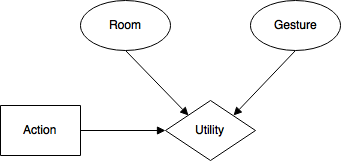
\includegraphics[width=0.50\textwidth]{images/influence-diagram}
\caption{Example model of the context engine using an influence diagram.}
\label{fig:evaluation:alternative-models:influence-diagram}
\end{figure}

Due to inference in the probabilistic network, actions are assigned a utility when we have soft or hard evidence on the gesture and room nodes. The utility of an action is shown with dark green bars below the name of the action in \Cref{fig:evaluation:alternative-models:hugin-influence-diagram}. For example, the utility of the \emph{Shelves\_Lamp\_Toggle} is 6682, making it the action with the highest utility and thus the action we decide to trigger\footnote{More information on influence diagrams in Hugin is available at \url{http://www.hugin.com/technology/getting-started/ids}}.

The scenario previously discussed in \Cref{sec:evaluation:user-tests} in which an incorrect action was triggered because a gesture is associated with multiple actions and thus those actions get a belief is shown in an influence diagram in \Cref{fig:evaluation:alternative-models:hugin-influence-diagram}. In contrast to the model based on a Bayesian network, the correct action can be triggered with greater confidence when utilizing the influence diagram.

When testing the Bayesian network with a subset of the recorded data during the user tests, we found that when using the influence diagram, we were able to more often trigger the correct action. During the user test, participant 7 a correct action was triggered 36\% of the time. Using the exact same beliefs on gesture and room nodes in the influence diagram, the correct action is triggered 50\% of the time.

% Note that during the tests with the Bayesian network we considered the outcome of performing an action acceptable if a list of suggested actions were shown and the intended action was in the list. This was not taken into account when testing the influence diagram with the data from participant 7 and as such the accuracy of the influence diagram may increase if a threshold for the utility of accepted actions is introduced.

\begin{figure}[h]
\centering
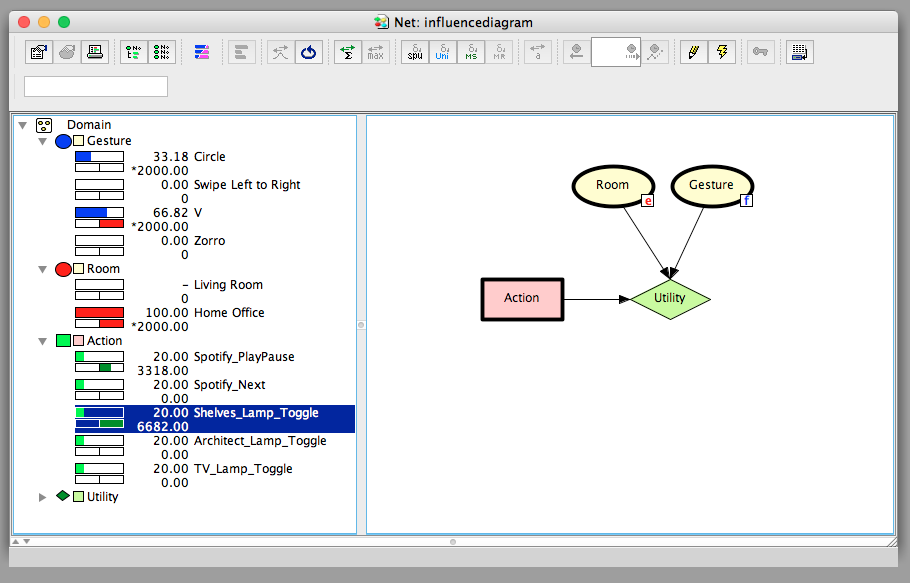
\includegraphics[width=\textwidth]{images/hugin-influence-diagram}
\caption{Screenshot of example influence diagram in Hugin. The screenshot shows that the influence diagram solves the problem of a single gesture being bound to multiple actions, can result in an incorrect action being triggered because the belief is reduced as shown in \Cref{table:participant-2-first-run} and discussed in \Cref{sec:evaluation:user-tests}.}
\label{fig:evaluation:alternative-models:hugin-influence-diagram}
\end{figure}

\subsection{Calculation of Gesture Beliefs}

In \Cref{sec:design:bayesian-network:gesture-node-evidence} the computation of beliefs on the Gesture node in the Bayesian network is specified. We only consider gesture templates with a score of 70 or below and then compute the average score. We found that this approach may cause issues, because a single gesture template may have a very low score but all other gesture templates with the same name have very high scores, thus the single gesture template is an outlier potentially causing us to consider an incorrect gesture recognized.

Instead we propose computing the average before filtering the gesture templates. Naturally, the average of each gesture will be larger as we include templates with a higher score in the computation and as such the threshold for accepted gesture should be higher.

Using the scores of the gestures performed by participant 7 in the user test, we computed how many actions would be correctly triggered when computing the average of the scores first and then filter them based on a threshold. We chose a threshold of 100. We found that 45\% of the actions were correctly triggered when we adjusted the computations of the gesture beliefs. This is in contrary to 41\% before the adjustments were made. While the adjustments are not a big impact, this can be considered an indication that the computations of beliefs in the Gesture node should have been performed differently.

We also found that when changing the way we compute beliefs for the Gesture node, we are generally able to put a greater belief on the correct action. This is examplified in \Cref{sec:evaluation:alternative-models:improved-action-beliefs}. The beliefs are taken from a scenario where the user desires to trigger the \emph{Spotify\_PlayPause} action. Note that in the beliefs before the improvements to the computations, \emph{Spotify\_Next} has the greatest belief where as after the improvements are made, the \emph{Spotify\_PlayPause} has the highest belief.
The average score used when computing the improved beliefs are shown in \Cref{sec:evaluation:alternative-models:improved-gesture-beliefs}. Note that only the Circle and V gestures have an average score below 100 and thus only those two gestures are assigned a belief greater than zero. Before improving the computations, all four gestures were assigned a belief greater than zero.

\begin{table}[]
\centering
\caption{Example beliefs of the Gesture node for participant 7 when attempting to trigger an action. The beliefs are shown before the computations were improved and after.}
\label{sec:evaluation:alternative-models:improved-action-beliefs}
\begin{tabular}{lll}
\textbf{Action}         & \textbf{Belief before} & \textbf{Belief after} \\
Spotify\_PlayPause      & 28.39                                              & 42.24                                             \\
Spotify\_Next           & 30.06                                              & 16.67                                             \\
Shelves\_Lamp\_Toggle   & 22.87                                              & 28.88                                             \\
Architect\_Lamp\_Toggle & 6.20                                               & 12.21                                             \\
TV\_Lamp\_Toggle        & 12.48                                              & 0                                                 
\end{tabular}
\end{table}

\begin{table}[]
\centering
AA\caption{Average scores of gestures used when computing the beliefs for the ``Belief after'' column shown in \Cref{sec:evaluation:alternative-models:improved-beliefs}.}
\label{sec:evaluation:alternative-models:improved-gesture-beliefs}
\begin{tabular}{ll}
\textbf{Gesture}    & \textbf{Score} \\
Circle              & 89.80          \\
Swipe Left to Right & 116.03         \\
V                   & 94.03          \\
Zorro               & 110.54         
\end{tabular}
\end{table}

%%% Local Variables:
%%% mode: latex
%%% TeX-master: "../../master"
%%% End:
